\documentclass[portuguese,oneside]{UFFStex}

% Para inserção de figuras.
\usepackage{graphicx}
\usepackage{pdflscape}
% Para tabelas com elementos ocupando mais de uma linha
\usepackage{multirow}
% Para inserir figuras lado a lado.
 \usepackage{subfigure}
% Para formatar algoritmos.
\usepackage{algorithmic}
\usepackage[portuguese,algo2e,boxruled]{algorithm2e}
% Hyperlink em capitulos, seções, citações
\usepackage[hidelinks]{hyperref}
% Bibliografia e citações padrão ABNT
%https://mirrors.ibiblio.org/CTAN/macros/latex/contrib/abntex2/doc/abntex2cite-alf.pdf
% Comandos: \citeonline{ref} \citeauthor{ref} \citeyear{ref}
%\usepackage[num]{abntex2cite}	% numérica
\usepackage[alf]{abntex2cite}	% alfabetica
% Referência cruzada que já coloca o tipo (Tabela, Figura, etc)
\usepackage[brazilian]{cleveref} 
% Pacote para revisão de texto
\setlength {\marginparwidth }{2cm}
\usepackage{easyReview}
\usepackage{booktabs}

% Autor
\author{Luiz Fernando Klein}

% Título português e inglês
\title{Comparação de bancos de dados de série temporal}
      {Comparison of time series databases}

% Tipo de trabalho
\tipotrabalho{\tci}         % Trabalho de Conclusão I
%\tipotrabalho{\tcii}        % Trabalho de Conclusão II

% Curso
\curso{\cc} % Ciência da Computação

% Orientador
\orientador{Geomar Schreiner}

% Palavras chave e Keywords (min 1, max 5, comma-separated)
\palavraschave{Banco de dados, Séries temporais, TimescaleDB, InfluxDB, Apache IoTDB}
              {Database, Time series, TimescaleDB, InfluxDB, Apache IoTDB}

\begin{document}

%----------------------------------------------------------------
% Ficha catalográfica (OBRIGATÓRIO para TCC II)
%  Você pode gerar a ficha neste link também: 
%   https://ficha.uffs.edu.br/
%----------------------------------------------------------------
\fichacatalografica

%----------------------------------------------------------------
% Folha de aprovação (OBRIGATÓRIO para TCC II)
%   Primeiro parâmetro é a data da defesa
%   Demais parâmetros são os membros da banca (pelo menos 2 nomes)
%   Não precisa passar o nome do Orientador
%----------------------------------------------------------------
\folhadeaprovacao{XX/12/2025}{Denio Duarte - UFFS}{Giancarlo Salton - UFFS}{}


%----------------------------------------------------------------
% Depois da folha de aprovação vem a dedicatória e a epígrafe.
%----------------------------------------------------------------
%\dedigrafe{Dedico este trabalho a meus pais.}
%          {The art of simplicity is a puzzle of complexity.}
%          {Douglas Horton}

% Resumo
\begin{resumo}
Este trabalho propõe uma revisão bibliográfica sobre bancos de dados de séries temporais (TSDBs), com foco em desempenho, arquitetura e aplicações práticas. O estudo visa analisar trabalhos comparativos entre sistemas como PostgreSQL, InfluxDB, TimescaleDB e Apache IoTDB, abordando métricas como taxa de ingestão, latência em consultas e consumo de recursos. A pesquisa explorará a adequação de diferentes TSDBs para cenários específicos, como IoT, edge computing e cloud, utilizando tanto conjuntos de dados reais quanto sintéticos. Ferramentas de benchmark consolidadas e soluções personalizadas serão avaliadas para compor as metodologias de teste. O objetivo é identificar padrões e lacunas na literatura, fornecendo um fundamento para futuras implementações e pesquisas na área.
\end{resumo}

% Abstract
\begin{abstract}
This work proposes a literature review on time-series databases (TSDBs), focusing on performance, architecture, and practical applications. The study aims to analyze comparative research on systems such as PostgreSQL, InfluxDB, TimescaleDB, and Apache IoTDB, covering metrics like ingestion rates, query latency, and resource usage. The research will explore the suitability of different TSDBs for specific scenarios, including IoT, edge computing, and cloud, using both real and synthetic datasets. Established benchmark tools and custom solutions will be evaluated for testing methodologies. The goal is to identify patterns and gaps in the literature, providing a foundation for future implementations and research in the field.
\end{abstract}

% Listas e sumário, nessa ordem. Somente o sumário é obrigatório.
\listoffigures       % Lista de figuras      (OPCIONAL)
\listoftables        % Lista de tabelas      (OPCIONAL)
% \listofalgorithms    % Lista de algoritmos   (OPCIONAL)
% \listofacronyms      % Lista de siglas       (OPCIONAL)
% \listofsymbols       % Lista de símbolos     (OPCIONAL)
\tableofcontents     % Sumário               (OBRIGATÓRIO)

% Desenvolvimento
\chapter{Introdução}
\label{chap:intro}

A crescente adoção de tecnologias como Internet das Coisas (IoT), sistemas de monitoramento industrial e aplicações financeiras em tempo real tem gerado um volume sem precedentes de dados temporais, criando desafios críticos para infraestruturas de armazenamento e análise.

\begin{figure}[h]
    \centering
    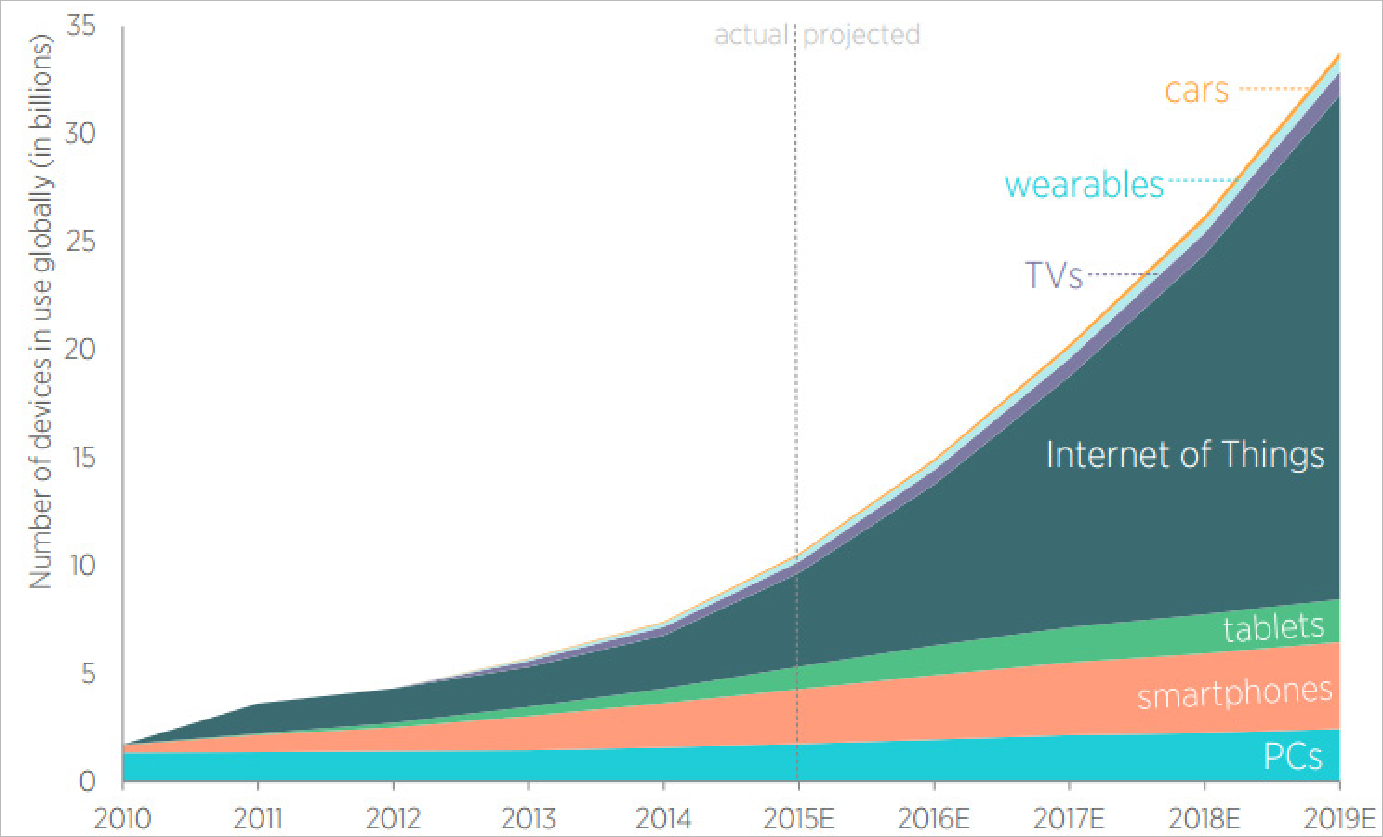
\includegraphics[width=1\textwidth]{figuras/projecao-iot.png}
    \caption{IoT: Dispositivos em uso globalmente}
    \label{fig:projecao_iot}
\end{figure}

A Figura \ref{fig:projecao_iot}, de \citeonline{thierer2015iot}, demonstra que, com a revolução digital, uma explosão na geração de dados temporais vem transformando profundamente a maneira como organizações coletam, armazenam e analisam informações. O gráfico também sugere que o número de dispositivos IoT conectados deve aumentar ainda mais nos próximos anos.

Segundo \citeonline{palma2016}, diversos setores passaram a depender da capacidade de processar fluxos contínuos de dados. Entre eles, destacam-se: o setor financeiro, que utiliza essa tecnologia para analisar flutuações de ações e volumes de transações; o de serviços de transporte, que a emprega no monitoramento de viagens e migrações sazonais; o da medicina, para acompanhar a disseminação de doenças e vírus; e o da análise meteorológica, que permite o uso de dados históricos para previsões mais precisas.

Esses fluxos são sequências de eventos ou medições que são naturalmente ordenadas e indexadas pelo tempo, com precisão de milissegundos. Essa avalanche de informações sequenciais expôs as limitações fundamentais dos bancos de dados tradicionais quando confrontados com padrões de acesso temporal, ingestão em alta velocidade e armazenamento eficiente de históricos de longo prazo.

Neste cenário desafiador, os bancos de dados de séries temporais (TSDBs) emergiram como soluções especializadas, arquitetadas desde sua concepção para atender às exigências únicas dos dados temporais. Ao contrário dos sistemas de propósito geral, os TSDBs incorporam em seu núcleo mecanismos otimizados para compressão temporal, indexação baseada em intervalos e processamento eficiente de operações temporais.

Bancos de dados de séries temporais (TSDBs) como o InfluxDB superam sistemas tradicionais em velocidade e eficiência ao lidar com dados indexados pelo tempo. \citeonline{naqvi2017influxdb} argumenta que bancos relacionais sofrem com problemas como indexação e falta de espaço em memória diante de um grande volume de dados temporais, enquanto TSDBs mantêm alta performance porque foram construídos para tratar o tempo como sua primeira preocupação.

Além da velocidade, os TSDBs oferecem compressão específica, co-localização de dados por intervalo de tempo e políticas de retenção automática que reduzem custos. Essas características tornam os bancos de séries temporais indispensáveis para aplicações de IoT, onde o fluxo contínuo de medições exige escalabilidade e uso econômico de recursos, superando limitações inerentes dos modelos tradicionais.

Propõe-se a realização de uma análise comparativa abrangente dos principais sistemas TSDBs atuais. O estudo avaliará critérios multidimensionais que incluem não apenas as métricas tradicionais de taxa de ingestão e latência de consulta, mas também aspectos quanto às funcionalidades oferecidas por cada uma das alternativas disponíveis e à consistência de manutenção e atualização dessas tecnologias por seus mantenedores.

A metodologia adotada neste estudo integrará abordagens distintas: a análise crítica de benchmarks publicados, destacando suas limitações metodológicas; uma série de experimentos controlados utilizando ferramentas de benchmarks para validar os achados teóricos em condições reproduzíveis e a avaliação do desenvolvimento, distribuição, documentação e suporte oferecido pelos proprietários. Os testes empíricos empregarão tanto conjuntos de dados sintéticos, permitindo o isolamento de variáveis específicas, quanto fluxos reais de produção industrial, garantindo a relevância prática dos resultados, enquanto as análises qualitativas se baseiam nos documentos disponibilizados, tanto por mantenedores, quanto pela comunidade dessas tecnologias.

Como resultado, esta pesquisa oferece um guia para aqueles que enfrentam o desafio de selecionar a solução ótima para seus contextos específicos. Em um mercado onde novas variantes de TSDBs surgem constantemente, cada uma prometendo vantagens específicas, este trabalho busca fornecer informações úteis e detalhadas para a tomada de decisão informada, fundamentada em evidências quantitativas e qualitativas.

\section{Objetivos Gerais}

O objetivo principal deste estudo é realizar uma análise comparativa abrangente dos principais bancos de dados de séries temporais disponíveis atualmente, avaliando seu desempenho, funcionalidades e adequação a diferentes cenários de aplicação, com o intuito de fornecer um referencial técnico para auxiliar na seleção da solução mais apropriada conforme os requisitos específicos de cada projeto.

\section{Objetivos Específicos}

\begin{itemize}
    \item Examinar metodologias de avaliação de estudos comparativos prévios.
    \item Avaliar a validade experimental e reprodutibilidade dos resultados encontrados.
    \item Realizar testes controlados com os principais bancos de dados temporais.
    \item Medir desempenho em ingestão, consultas complexas e consumo de recursos.
    \item Utilizar dados sintéticos e reais para comparação em diferentes cenários.
    \item Analisar funcionalidades e serviços disponíveis nos bancos de dados que melhor performaram.
    \item Consolidar achados em tabela comparativa para auxiliar na seleção de TSDBs.
\end{itemize}

\section{Justificativa}

A utilização de bancos de dados tradicionais para armazenamento de séries temporais resulta em problemas concretos: baixo desempenho na ingestão de dados em alta velocidade, consultas temporais ineficientes, consumo excessivo de recursos computacionais e custos elevados devido à falta de mecanismos de compressão temporal especializados. Esse cenário expõe as limitações dos bancos de dados tradicionais no tratamento eficiente desses fluxos contínuos de informação marcada temporalmente, justificando a necessidade de soluções especializadas.

A relevância desta pesquisa se fundamenta em dois pilares principais. Primeiramente, a carência de estudos comparativos abrangentes que considerem simultaneamente aspectos de desempenho e adequação a domínios específicos de aplicação. Enquanto diversos trabalhos analisam métricas isoladas, poucos oferecem uma visão holística que auxilie decisões tecnológicas em projetos reais. Em segundo lugar, a velocidade de evolução desses sistemas, com novas versões e funcionalidades sendo lançadas constantemente, torna obsoletas muitas comparações existentes após curtos períodos.

Do ponto de vista prático, a seleção inadequada de um banco de dados temporal pode acarretar custos operacionais significativos. A migração de um sistema relacional tradicional para um TSDB especializado pode reduzir em diversas vezes os custos de infraestrutura para armazenamento e processamento de dados. Este trabalho busca fornecer critérios objetivos para uma avaliação comparativa.

Além disso, a pesquisa contribui para a consolidação de metodologias de avaliação de bancos de dados temporais, área ainda carente de padrões consolidados. A proposta de uma comparação, que integre métricas quantitativas e qualitativas, representa uma inovação potencial para futuros estudos na área. Adicionalmente, a disponibilização pública dos \textit{scripts} e configurações utilizadas nos experimentos visa suprir uma lacuna importante na literatura atual: a reprodutibilidade dos resultados comparativos.
\chapter{Referencial Teórico}

Este capítulo apresenta os conceitos fundamentais que embasam a pesquisa, organizados em quatro seções principais. Inicialmente, são abordados os conceitos gerais de bancos de dados e o modelo relacional, estabelecendo a base teórica necessária. Em seguida, são discutidos os bancos de dados distribuídos, essenciais para compreender a escalabilidade em ambientes modernos. Na sequência, são explorados os bancos de dados de séries temporais (TSDBs), foco central deste trabalho. Por fim, são apresentados os métodos de avaliação de desempenho através de benchmarks, fundamentais para a análise comparativa proposta.

\section{Banco de Dados}

Segundo \citeonline{Ramakrishnan2003}, um banco de dados pode ser definido por uma coleção de dados, tipicamente descrevendo as atividades de uma ou mais organizações relacionadas. Esta definição abrange desde informações sobre entidades, como estudantes e cursos em uma universidade, até os relacionamentos entre essas entidades, como a matrícula de alunos em disciplinas específicas. Em \citeonline{Silberschatz2020} argumenta-se ainda que o principal objetivo de um banco de dados deve ser fornecer uma maneira de recuperar informações que seja tanto conveniente quanto eficiente.

O gerenciamento desses dados é realizado por um Sistema de Gerenciamento de Banco de Dados (SGBD), que é um software projetado para auxiliar na manutenção e utilização de grandes coleções de dados \cite{Ramakrishnan2003}. Os autores destacam que a necessidade por tais sistemas tem crescido rapidamente, sendo a alternativa ao uso de um SGBD a adoção de abordagens ad-hoc que não são transferíveis de uma aplicação para outra, como armazenar os dados em arquivos e escrever código específico para gerenciá-los.

A importância dos bancos de dados na era da informação é ressaltada pelos autores quando afirmam que o sucesso de uma organização depende cada vez mais de sua capacidade de adquirir dados precisos e oportunos sobre suas operações, gerenciar esses dados efetivamente e usá-los para analisar e guiar suas atividades \citeonline{Ramakrishnan2003}. Esta afirmação reflete o papel central que os bancos de dados assumiram nas organizações modernas, onde a informação é reconhecida como um ativo estratégico.

\citeonline{Ramakrishnan2003} apresentam diversas vantagens no uso de um SGBD em comparação com sistemas de arquivos tradicionais. Entre elas destacam-se a independência de dados, que isola os programas aplicativos dos detalhes de representação e armazenamento; o acesso eficiente aos dados, possibilitado por técnicas sofisticadas de armazenamento e recuperação; a integridade e segurança dos dados, permitindo que o SGBD restrinja acessos não autorizados; e o suporte a acesso concorrente e recuperação após falhas.

O modelo relacional, proposto por Codd em 1970, revolucionou a área de bancos de dados e substituiu em grande parte os modelos hierárquico e de rede que o precederam. Segundo os autores, este modelo é simples e elegante, onde um banco de dados é visto como uma coleção de relações (tabelas com linhas e colunas), sendo que esta representação tabular permite até mesmo usuários iniciantes compreenderem facilmente os conteúdos armazenados \citeonline{Ramakrishnan2003}.

A estruturação dos dados no modelo relacional é baseada em relações, que consistem em um esquema da relação e uma instância da relação \citeonline{Ramakrishnan2003}. O esquema especifica o nome da relação, o nome de cada campo (ou coluna) e o domínio de cada campo, enquanto a instância é um conjunto de tuplas (registros) onde cada tupla possui o mesmo número de campos que o esquema da relação. Os autores enfatizam que cada relação é definida para ser um conjunto de tuplas únicas, o que garante a não duplicação de registros.

Para garantir a qualidade e consistência dos dados armazenados, os bancos de dados utilizam restrições de integridade (ICs), que são condições especificadas no esquema do banco de dados e que restringem os dados que podem ser armazenados em uma instância do banco de dados \citeonline{Ramakrishnan2003}. Quando uma instância de banco de dados satisfaz todas as restrições de integridade especificadas no esquema do banco de dados, dizemos que é uma instância legal, e o SGBD deve garantir que apenas instâncias legais sejam armazenadas.

Mesmo assim, é importante que o banco de dados ofereça para os usuários uma visão abstrata dos dados, ou seja, ocultando certos detalhes de como os dados são armazenados ou mantidos, argumenta \citeonline{Silberschatz2020}. Deve servir como abstração para resolução de problemas reais de maneira eficiente e prática.

Entre os principais tipos de restrições de integridade destacam-se as restrições de chave, que afirmam que um subconjunto mínimo dos campos de uma relação é um identificador único para uma tupla, e as restrições de chave estrangeira, que ocorrem quando a informação em uma relação está ligada à informação em outra relação. Estas restrições são fundamentais para manter a consistência dos dados quando múltiplas tabelas estão relacionadas.

A linguagem SQL tornou-se o padrão para interação com bancos de dados relacionais. Como observam \citeonline{Ramakrishnan2003}, SQL é a linguagem comercial mais popular para SGBDs relacionais. A linguagem permite não apenas a definição da estrutura dos dados, mas também sua manipulação e consulta, sendo que uma consulta ao banco de dados relacional é definida como uma pergunta sobre os dados, cuja resposta consiste em uma nova relação contendo o resultado.

O projeto de um banco de dados relacional frequentemente começa com um diagrama Entidade-Relacionamento (ER), que é conveniente para representar um projeto inicial de alto nível. Os autores descrevem um método padrão para traduzir um diagrama ER em um esquema de banco de dados relacional que se aproxima do projeto ER original, embora com algumas limitações na representação de certas restrições usando apenas SQL-92.

Em resumo, os bancos de dados representam a principal tecnologia para armazenamento e gerenciamento de informações nas organizações modernas, oferecendo vantagens significativas em termos de eficiência, segurança e consistência dos dados quando comparados a abordagens alternativas de armazenamento. O modelo relacional, com sua simplicidade e poder de expressão, consolidou-se como o paradigma dominante na área, sendo implementado pela maioria dos sistemas comerciais atuais.

\section{Bancos de Dados Distribuídos}

Os bancos de dados distribuídos (BDDs) representam a convergência entre duas tecnologias aparentemente opostas: sistemas de banco de dados e redes de computadores \citeonline{Ozsu2011}. Enquanto os sistemas de banco de dados tradicionais promovem a centralização dos dados para garantir controle e integridade, as redes de computadores incentivam a distribuição e descentralização. A tecnologia de BDDs sintetiza esses conceitos, demonstrando que a integração dos dados não necessariamente implica na sua centralização física.

Para \citeonline{Silberschatz2020}, de maneira similar, um sistema de banco de dados distribuído é composto por várias instâncias com bancos locais, capazes de processar transações locais. Também podem executar transações globais, que acessam dados em múltiplos sites, exigindo comunicação entre eles.

Um \textit{banco de dados distribuído} é definido como uma coleção de múltiplos bancos de dados logicamente inter-relacionados, distribuídos por uma rede de computadores \citeonline{Ozsu2011}. O sistema de gerenciamento de banco de dados distribuído (SGBDD) é o software que permite o gerenciamento desse banco de dados distribuído, tornando a distribuição transparente para os usuários. É importante destacar que um BDD não é simplesmente um conjunto de arquivos armazenados em diferentes nós de uma rede, mas sim um sistema estruturado com esquema definido e acesso através de uma interface comum.

A arquitetura de um SGBDD pode ser organizada de diferentes formas, sendo as principais: sistemas \textit{cliente/servidor}, sistemas \textit{peer-to-peer} (ponto-a-ponto) e sistemas \textit{multibanco de dados} \citeonline{Ozsu2011}. Nos sistemas cliente/servidor, as funções são divididas entre clientes (que gerenciam a interface com o usuário) e servidores (responsáveis pelo gerenciamento dos dados). Já nos sistemas peer-to-peer, todas as máquinas possuem funcionalidade completa de SGBD e podem se comunicar diretamente para executar consultas e transações. Os sistemas multibanco de dados lidam com a integração de bancos de dados heterogêneos e autônomos.

Uma das principais promessas dos BDDs é o gerenciamento transparente de dados distribuídos e replicados. Essa transparência se manifesta em vários níveis: independência de dados (imunidade das aplicações a mudanças na estrutura lógica ou física dos dados), transparência de rede (proteção do usuário contra detalhes operacionais da rede), transparência de replicação (ocultação da existência de cópias múltiplas dos dados) e transparência de fragmentação (divisão das relações em fragmentos tratados como objetos independentes). Como destacam \citeonline{Ozsu2011}, o objetivo mais importante da tecnologia de banco de dados é a integração, não a centralização.

\citeonline{Silberschatz2020} afirma que bancos de dados distribuídos podem ser homogêneos ou heterogêneos, que são, respectivamente, sistemas de banco de dados em que os esquemas ou código são comuns entre as instâncias ou que diferem entre cada instância.

Os BDDs oferecem maior confiabilidade através do suporte a transações distribuídas. Uma transação é definida como uma unidade básica de computação confiável e consistente, consistindo em uma sequência de operações de banco de dados executadas como uma ação atômica. Em um ambiente distribuído, as transações podem ser executadas em vários sites, acessando bancos de dados locais. Com suporte completo a transações distribuídas, os usuários podem acessar uma única imagem lógica do banco de dados, confiando no SGBDD para garantir que suas requisições serão executadas corretamente, independentemente de falhas no sistema.

O desempenho em BDDs pode ser melhorado através da localização dos dados (armazenamento próximo aos pontos de uso) e do aproveitamento do paralelismo inerente dos sistemas distribuídos. A localização reduz a contenção por serviços de CPU e E/S, enquanto o paralelismo pode ser explorado tanto entre consultas (\textit{inter-query}) quanto dentro de uma única consulta (\textit{intra-query}) \citeonline{Ozsu2011}. No entanto, como alertam \citeonline{Ozsu2011}, a mistura de operações de leitura e atualização requer a implementação de elaborados protocolos de controle de concorrência.

Entre os principais desafios dos BDDs estão a replicação de dados, o tratamento de falhas e a sincronização de transações em múltiplos sites. \citeonline{Silberschatz2020} aponta que a detecção de impasse em sistemas distribuídos exige cooperação entre sites, pois podem ocorrer impasses globais mesmo sem impasses locais.

A replicação introduz complexidade na manutenção da consistência entre as cópias dos dados. As falhas de sites ou enlaces de comunicação exigem mecanismos para garantir que os efeitos das atualizações sejam refletidos em todos os locais assim que o sistema se recuperar. Além disso, como cada site não tem informação instantânea sobre as ações que estão sendo executadas nos outros sites, a sincronização de transações se torna significativamente mais complexa do que em sistemas centralizados.

Os problemas de projeto em SGBDDs incluem: projeto do banco de dados distribuído (fragmentação e distribuição ótima dos dados), gerenciamento de diretórios distribuídos, processamento de consultas distribuídas, controle de concorrência distribuído, gerenciamento de deadlock distribuído, confiabilidade do SGBDD e protocolos de replicação . Como destacam \citeonline{Ozsu2011}, esses problemas não são isolados, mas sim inter-relacionados, onde a solução de um afeta os outros.

A arquitetura de referência para SGBDDs peer-to-peer, conforme apresentada por \citeonline{Ozsu2011}, inclui três níveis de esquema: esquema conceitual global (visão lógica de todos os dados no sistema), esquema conceitual local (organização lógica dos dados em cada site) e esquema interno local (organização física em cada site). Essa arquitetura é implementada através de dois componentes principais: o \textit{processador do usuário} (que lida com a interface do usuário, controle semântico, otimização de consultas e monitoramento de execução) e o \textit{processador de dados} (responsável pelo processamento local de consultas, gerenciamento de recuperação e suporte à execução).

Bancos de dados distribuídos representam uma evolução natural dos sistemas de banco de dados em um mundo cada vez mais conectado, oferecendo benefícios significativos em termos de transparência, confiabilidade e desempenho, mas também introduzindo complexidades adicionais no gerenciamento da distribuição dos dados e do processamento das transações.

\subsection{Bancos de Dados de Séries Temporais}

Os bancos de dados de séries temporais (TSDB - \textit{Time Series Databases}) representam uma categoria especializada de sistemas de armazenamento projetados para lidar com dados que são registrados como uma sequência de valores, cada um associado a um momento temporal específico. Segundo \citeonline{Ozsu2011}, uma série temporal é um conjunto de valores de atributos ao longo de um período de tempo. Essa característica fundamental diferencia os TSDBs dos bancos de dados tradicionais, pois eles são otimizados para consultas baseadas em intervalos de tempo, oferecendo desempenho superior para esse padrão de acesso.

Registros meteorológicos, indicadores econômicos e métricas de evolução da saúde do paciente — todos são dados de séries temporais. Dados de séries temporais também podem incluir métricas de servidor, monitoramento de desempenho de aplicativos, dados de rede, dados de sensores, eventos, cliques e muitos outros tipos de dados analíticos. \citeonline{InfluxDataTimeSeries}.

\begin{figure}[h]
    \centering
    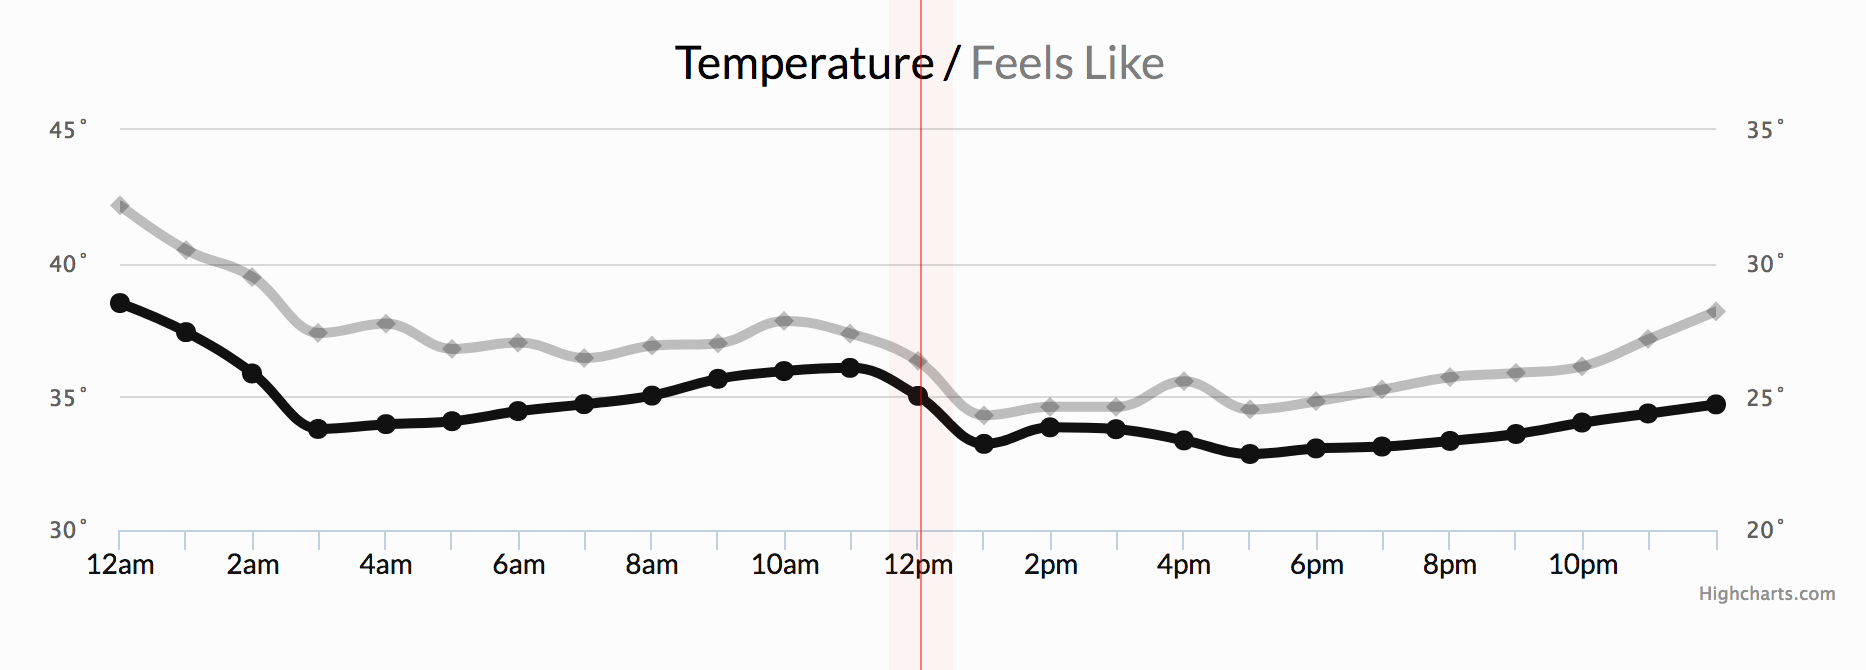
\includegraphics[width=0.7\textwidth]{figuras/dado_temporal.png}
    \caption{Exemplo de dado temporal: Condições meteorológicas}
    \label{fig:dado_temporal}
\end{figure}

\begin{figure}[h]
    \centering
    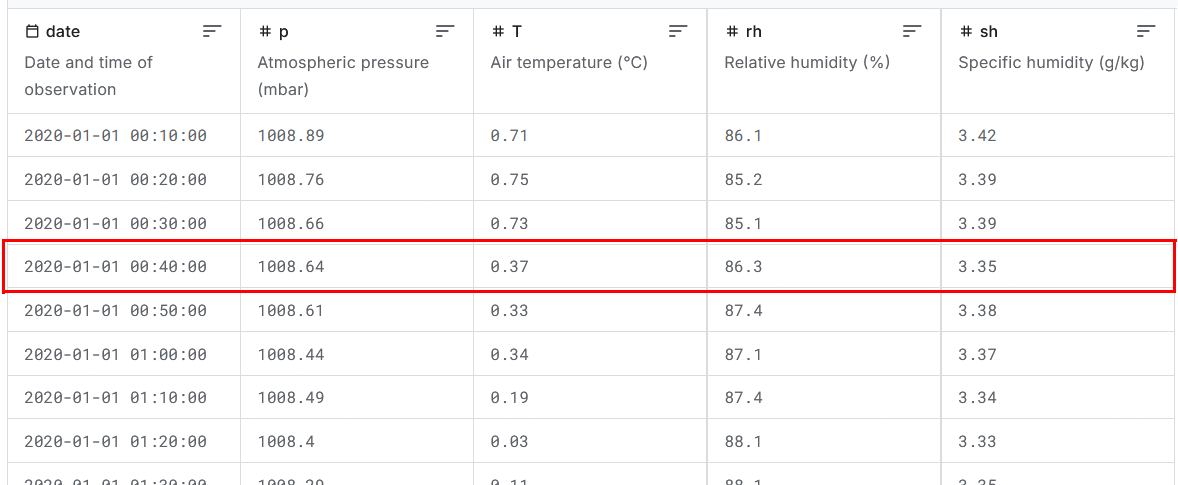
\includegraphics[width=1\textwidth]{figuras/registro_temporal.png}
    \caption{Exemplo de registro de dado temporal em um TSDB}
    \label{fig:registro_temporal}
\end{figure}

A Figura \ref{fig:dado_temporal} apresenta uma série temporal de condições meteorológicas. O elemento destacado em vermelho dentro do gráfico corresponde a um dado temporal único, um registro individual no TSDB capturado pelo sensor naquele instante.

Já a Figura \ref{fig:registro_temporal} apresenta uma tabela de um TSDB, representando a série temporal de condições meteorológicas. O elemento destacado em vermelho na tabela corresponde a um registro de um dado temporal único, com informações de data e hora, pressão atmosférica, temperatura do ar, umidade, entre outros.

Conforme explicado por \citeonline{Ozsu2011}, normalmente, uma série temporal consiste apenas em valores numéricos, sejam eles contínuos ou discretos. Consequentemente, é possível modelar fluxos de dados que contêm apenas valores numéricos como séries temporais. Isso permite usar técnicas de análise que foram desenvolvidas para séries temporais em alguns tipos de fluxo de dados. Uma característica importante é que os conjuntos de dados de séries temporais são normalmente usados em situações em que as medições, uma vez feitas, não são revisadas ou atualizadas, mas sim acumuladas, com novos dados adicionados para cada parâmetro medido em cada novo ponto no tempo \citeonline{Dunning2014}.

A importância histórica das séries temporais é notável, com exemplos que remontam ao século XIX. \citeonline{Dunning2014} mencionam o trabalho pioneiro de Matthew Fontaine Maury, que analisou registros de navios para criar cartas de ventos e correntes, demonstrando como a análise coletiva de dados de séries temporais acumulados ao longo de muitos anos em diários de bordo de muitos navios poderia revelar padrões valiosos para a navegação marítima. Esse exemplo histórico ilustra como os conjuntos de dados de séries temporais podem revelar tendências e padrões que não são aparentes em medições pontuais.

No contexto moderno, os TSDBs enfrentam novos desafios devido ao volume, velocidade e variedade dos dados gerados. Como observam \citeonline{Dunning2014}, o que antes era coletado em 10 minutos para alguns sistemas muito ativos agora é gerado a cada segundo. Essa explosão na quantidade de dados exige novas abordagens para armazenamento e acesso, tornando os bancos de dados NoSQL particularmente adequados para essa tarefa. Os autores argumentam que para consultas baseadas em tempo em escalas muito grandes, os acessos baseados em tempo podem ser implementados como varreduras grandes e contíguas que são muito eficientes se os dados forem armazenados adequadamente em um banco de dados de séries temporais.

A arquitetura dos TSDBs modernos evoluiu significativamente. \citeonline{Dunning2014} descrevem três abordagens principais para o armazenamento de séries temporais: (1) tabelas largas (\textit{wide tables}) que armazenam os dados ponto a ponto, (2) design híbrido que mistura tabelas largas com armazenamento em blobs, e (3) inserção direta de blobs a partir de um cache na memória. A abordagem de inserção direta de blobs é particularmente interessante, pois permite taxas de ingestão que podem ser até 1.000 vezes mais rápidas do que o sistema era capaz de ingerir dados sem a inserção direta de blobs.

As aplicações dos TSDBs são diversas e crescentes. \citeonline{Dunning2014} destacam casos de uso em setores como negociação de ações, telecomunicações, monitoramento de data centers e manutenção preditiva. Na área financeira, por exemplo, os autores observam que a velocidade das negociações e, portanto, a coleta de dados de negociação e a necessidade em muitos casos de latência extremamente pequena tornam o uso de bancos de dados de séries temporais de alto desempenho extremamente importante. Já no contexto da Internet das Coisas (IoT), os TSDBs ocupam uma posição central, pois ficam no coração do fluxo de dados de sensor para insight que está mudando rapidamente a maneira como percebemos e entendemos o mundo ao nosso redor.

Uma característica fundamental dos TSDBs é sua otimização para padrões específicos de consulta. Como explicam \citeonline{Dunning2014}, um banco de dados de séries temporais é uma maneira de armazenar várias séries temporais de forma que as consultas para recuperar dados de uma ou algumas séries temporais para um intervalo de tempo específico sejam particularmente eficientes. Essa eficiência é alcançada através de estratégias de armazenamento que agrupam dados temporais próximos fisicamente no armazenamento, permitindo operações de varredura sequencial eficientes.

A evolução dos TSDBs continua com o desenvolvimento de novas capacidades, como bancos de dados geo-temporais que incorporam informações de localização além do tempo. \citeonline{Dunning2014} preveem que a combinação de escala cada vez maior e mais tecnologias emergentes para coletar e analisar dados para insights valiosos está criando o desejo e a capacidade de fazer coisas novas. Essa visão aponta para um futuro onde os TSDBs desempenharão um papel ainda mais central na análise de dados em diversos domínios aplicados.

\section{Benchmarks}

A avaliação de desempenho constitui um aspecto crucial no processo de seleção de sistemas de gerenciamento de banco de dados. Conforme destacado por \citeonline{Ramakrishnan2003}, quando um banco de dados atinge dimensões que ultrapassam a capacidade do SGBD atual em fornecer desempenho satisfatório, mesmo com o melhor projeto possível, torna-se necessário considerar a migração para um novo sistema. Neste contexto, os benchmarks emergem como ferramentas essenciais para permitir comparações objetivas entre diferentes produtos disponíveis no mercado.

\citeonline{Silberschatz2020} argumenta sobre a importância de realizar testes de benchmark específicos para cada caso de uso. Como um único teste não é suficiente, utiliza-se um benchmark que simula cargas de trabalho reais, já que cada produto pode ter desempenho variado conforme a tarefa.

A complexidade inerente aos SGBDs e as diferentes abordagens adotadas pelos fornecedores tornam os benchmarks particularmente valiosos. Como observam \citeonline{Ramakrishnan2003}, um SGBD é um software complexo, e diferentes fornecedores podem direcionar seus sistemas para diferentes segmentos de mercado, colocando mais esforço em otimizar certas partes do sistema ou escolhendo diferentes projetos de sistema. Esta diversidade de enfoques e otimizações específicas dificulta a comparação direta entre sistemas, tornando os benchmarks padronizados instrumentos indispensáveis para auxiliar os usuários na seleção de um SGBD adequado às suas necessidades particulares.

No que diz respeito às características fundamentais de um bom benchmark, \citeonline{Ramakrishnan2003} enumeram três qualidades essenciais. Em primeiro lugar, a portabilidade, que se refere à capacidade do benchmark de ser executado em diferentes plataformas e sistemas. Em segundo lugar, a clareza, que garante a fácil compreensão do que está sendo efetivamente medido. Por fim, a escalabilidade, que permite a adaptação natural a instâncias maiores do problema. Além desses atributos básicos, os benchmarks ideais devem ser capazes de medir tanto o desempenho máximo, expresso em métricas como transações por segundo, quanto a relação custo-benefício, calculada em termos como dólar por transação por segundo, para cargas de trabalho típicas em um determinado domínio de aplicação. Foi precisamente para atender a essas necessidades que o Transaction Processing Council (TPC) foi criado, com a missão específica de desenvolver benchmarks padronizados para sistemas de processamento de transações e bancos de dados.

Além disso, \citeonline{Silberschatz2020} complementa que é importante calcular corretamente o desempenho médio: usar a média simples de throughputs pode induzir ao erro. O método adequado é calcular o tempo total para executar uma carga mista e, a partir disso, obter o throughput médio ou usar a média harmônica, que reflete melhor a realidade quando há diferentes tipos de transações.

A literatura especializada, conforme apresentada por \citeonline{Ramakrishnan2003}, categoriza os principais benchmarks disponíveis no mercado em três grupos principais. O primeiro grupo compreende os benchmarks de processamento de transações on-line, dentre os quais se destacam o TPC-A e TPC-B, que estabelecem as definições padrão para medidas de transações por segundo e custo por transação. Enquanto o TPC-A avalia o desempenho de toda uma rede de computadores incluindo o SGBD, o TPC-B concentra-se especificamente no sistema de gerenciamento de banco de dados. O TPC-C, por sua vez, representa uma evolução significativa em relação aos seus predecessores, modelando um ambiente complexo de armazém que rastreia itens fornecidos aos clientes através de cinco tipos diferentes de transações. Como explicam os autores, cada transação TPC-C é muito mais cara que uma transação TPC-A ou TPC-B, e o TPC-C exercita uma gama muito mais ampla de capacidades do sistema, o que levou este benchmark a substituir amplamente os anteriores como padrão para avaliação de processamento de transações.

O segundo grupo importante de benchmarks é dedicado especificamente à avaliação de desempenho em consultas. Nesta categoria, o Benchmark Wisconsin se destaca como ferramenta amplamente utilizada para medir o desempenho de consultas relacionais simples. Para cenários mais complexos, o Benchmark Set Query oferece avaliação de desempenho para um conjunto de consultas mais sofisticadas, enquanto o Benchmark AS3AP se especializa em medir o desempenho de cargas mistas que incluem transações, consultas relacionais e funções utilitárias. O TPC-D merece menção especial por constituir uma suíte abrangente de consultas SQL complexas, especialmente projetadas para representar o domínio de aplicação de suporte à decisão. Complementando esta categoria, o Benchmark do OLAP Council foi desenvolvido especificamente para avaliar consultas complexas de suporte à decisão, incluindo algumas que não podem ser expressas facilmente em SQL, sendo particularmente adequado para sistemas de processamento analítico on-line (OLAP).

O terceiro grupo identificado por \citeonline{Ramakrishnan2003} engloba os benchmarks especializados para bancos de dados de objetos. Neste domínio, os Benchmarks 001 e 007 foram concebidos especificamente para medir o desempenho de sistemas de banco de dados orientados a objetos, enquanto o Benchmark Bucky foi desenvolvido para avaliar sistemas de banco de dados objeto-relacionais, representando uma ponte entre os paradigmas relacional e orientado a objetos.

Quanto à utilização adequada desses benchmarks na prática, \citeonline{Ramakrishnan2003} oferecem diretrizes valiosas para garantir que os resultados sejam interpretados corretamente. A primeira consideração diz respeito à relevância do benchmark em si, alertando que métricas que tentam resumir o desempenho em um único número podem ser excessivamente simplistas, dado que um SGBD é um software complexo utilizado em diversas aplicações. Um bom benchmark deve, portanto, incluir uma suíte abrangente de tarefas cuidadosamente selecionadas para cobrir um domínio de aplicação específico e testar os recursos do SGBD que são críticos para aquele domínio. A segunda diretriz enfatiza a importância de analisar quão bem o benchmark reflete a carga de trabalho real do ambiente onde o SGBD será utilizado, recomendando que se dê maior peso ao desempenho nas tarefas do benchmark que mais se assemelham às operações críticas da aplicação pretendida. Finalmente, os autores sugerem a criação de benchmarks personalizados, adaptando benchmarks padrão ou substituindo suas tarefas por operações mais representativas da carga de trabalho específica do usuário, como forma de contornar possíveis otimizações específicas que os fornecedores possam ter implementado para obter bons resultados nos testes padronizados.
\chapter{Trabalhos Relacionados}

Para a elaboração deste estudo, foram revisados e analisados trabalhos de benchmarks e comparações, tanto de performance quanto de funcionalidades, de bancos de dados de séries temporais. A busca por trabalhos relacionados foi realizada utilizando as palavras-chave "data streaming", "timeseries" e "timeseries databases". Os resultados foram ordenados por quantidade de citações por trabalho, o que possibilitou uma seleção de análises mais elaboradas e desenvolvidas. Após a ordenação, selecionaram-se 23 resultados para leitura inicial, a fim de verificar a relevância para os objetivos deste estudo.

Dentre os 23 trabalhos, alguns não apresentaram relação direta suficiente para uma análise aprofundada, embora tenham fornecido informações relevantes para a construção deste estudo. \citeonline{zubaroglu2021data}, por exemplo, apresenta uma lista de datasets para serem utilizados em análises de bancos de dados de séries temporais. \citeonline{Gaber2005Mining} também foi outro trabalho que, apesar de não ter relação direta com o objetivo desta análise, trouxe muitas informações relevantes sobre os algoritmos usados pelos SGBDs de séries temporais apresentados.

Da primeira etapa de revisão, seis trabalhos dos vinte e três foram selecionados para um estudo detalhado. As informações deste capítulo referem-se a esses seis estudos.

Este capítulo está organizado em três seções principais. A seção de \textit{Análise de funcionalidades} agrega trabalhos que avaliam características técnicas e operacionais dos sistemas. A seção de \textit{Análise de performance} reúne estudos comparativos baseados em benchmarks e métricas de desempenho. Por fim, a \textit{Análise comparativa} sintetiza e critica os trabalhos selecionados por meio de uma tabela comparativa desenvolvida para este estudo, destacando padrões, lacunas e tendências identificadas na literatura.

\section{Análise de funcionalidades}

\citeonline{Petre2019} apresenta a relação dos bancos de dados com as funcionalidades apresentadas por cada um. Requisitos funcionais, que são aparentes ao usuário final, como uma funcionalidade específica, e requisitos não funcionais, como estratégias de compressão ou otimização de pesquisas, que não são aparentes ao usuário, mas que impactam diretamente na usabilidade.

O trabalho compara seis bancos de dados de séries temporais (TSDBs) de código aberto: InfluxDB, Graphite, RRDTool, Prometheus, OpenTSDB e TimescaleDB. O estudo avalia 18 atributos quantitativos e qualitativos, como desenvolvimento ativo, velocidade de desenvolvimento, maturidade de mercado, replicação de dados e suporte a bibliotecas, para classificar as soluções. O objetivo é auxiliar na seleção da TSDB mais adequada para as necessidades empresariais, considerando aspectos técnicos e operacionais. O resultado destacou o InfluxDB como a solução líder na análise.

\section{Análise de performance}

Para a próxima etapa da análise, foram selecionados 5 trabalhos no formato de benchmark ou, pelo menos, com comparações de desempenho em cenários reais e/ou sintéticos.

\citeonline{lima2024avaliando} utilizou testes de inserção (1.000 a 5 milhões de registros) e consultas agregadas com dados fictícios (medições de timestamp, local, temperatura e umidade) para comparar o desempenho entre SGBDs, executados via Apache JMeter. A mesma estrutura de dados foi replicada em todos os bancos, testando volumes de 500.000 e 5 milhões de registros. O ambiente empregou containers Docker para os SGBDs e JMeter, porém sem detalhes completos para reprodução. Os testes foram realizados em uma máquina com AMD Ryzen 5 4500, 16GB RAM e SSD, utilizando containers Docker locais. O InfluxDB foi o banco de dados que mais se destacou na pesquisa.

\citeonline{shah2022performance} comparou o desempenho de InfluxDB v2.1, TimescaleDB v2.6, Druid v0.22.1 e Cassandra v3.11.12 em operações de inserção e oito tipos de consultas (pontuais, agregações, etc.), avaliando tempo de carga, consumo de espaço e latência. Foram utilizados datasets reais (IoT, financeiro e NYC Taxi) e sintéticos (gerados via timeseries-generator em Python), sem menção a ferramentas externas como JMeter. O ambiente de testes consistiu em um Intel Core i5-9500 (6 núcleos), 8GB RAM, SSD 500GB e Ubuntu 20.04, com configurações de ambiente detalhadas. O banco de dados que mais se destacou foi o InfluxDB, não apenas em performance de consultas, mas também se saiu bem em consumo de espaço, ficando atrás apenas do Druid.

\citeonline{naqvi2017influxdb} comparou o desempenho do InfluxDB, SQL Server, Cassandra, Elasticsearch e OpenTSDB em três métricas principais: taxa de ingestão de dados, requisitos de armazenamento e tempo médio de resposta a consultas. Foram utilizados dados sintéticos (simulando métricas de servidores) e um dataset real de viagens de táxi de NYC (2009-2017), processados com ferramentas nativas dos SGBDs e scripts personalizados em Java. Os testes foram realizados em um ambiente com Intel Core i5-6300HQ (4 núcleos), 16GB RAM e SSD, em sistemas Windows 10 e Ubuntu 20.04, utilizando versões específicas dos bancos (como InfluxDB 1.3 e Elasticsearch 5.6.3). O estudo conclui que o InfluxDB é ideal para cenários de alta ingestão de dados temporais, como IoT e monitoramento, mas pode não ser adequado para aplicações que exigem operações complexas de JOIN ou atualizações frequentes.

\citeonline{pereira2023mulletbench} avaliou o desempenho de InfluxDB 2.7 e Apache IoTDB 1.1.1 em três cenários distintos (Cloud-only, 2 Edge + Cloud e 4 Edge + Cloud), testando cargas de inserção, consulta e mista, com cada teste executado 3 vezes após reinicialização. As ferramentas utilizadas incluíram o MulletBench para benchmark, Ansible + Docker para orquestração, PCP para monitoramento e tcconfig para simulação de rede. Os testes foram realizados em nós com Intel i5-9500 (16GB RAM, NVMe SSD) e clientes com Intel i3-4170 (16GB RAM, SATA SSD), em rede Gigabit comutada. As configurações detalhadas e o código estão disponíveis no GitHub do MulletBench e no Apêndice A. O Apache IoTDB se destacou na pesquisa.

\citeonline{wang2023iotdb} comparou o desempenho do IoTDB v0.13.0 com outros sistemas (InfluxDB, TimescaleDB, KairosDB, Parquet e ORC) em operações de escrita, leitura, custo de armazenamento e consultas (range, agregação, downsampling), medindo throughput, latência e tempo de resposta. Foram utilizados datasets industriais reais (dados de veículos, trens e máquinas) e sintéticos (gerados pelo TSBS), sem ferramentas externas além do TSBS. Os testes foram realizados em ambientes stand-alone (Intel i7-10700, 32GB RAM, 10TB HDD) e distribuídos (Alibaba Cloud com Xeon Platinum, 256GB RAM), com configurações específicas como replicação fator 3 e particionamento temporal. Detalhes das configurações estão no texto, mas não há um guia completo de reprodução. Na análise do trabalho, o Apache IoTDB demonstrou superioridade tanto em ambientes locais quanto distribuídos, especialmente em larga escala, como em aplicações industriais com trilhões de pontos de dados.

\section{Análise comparativa}

Após análise minuciosa, foi desenvolvida a Tabela \ref{tab:comparacoes}  para agregar informações úteis e possibilitar análises comparativas entre os trabalhos que possuem análise de performance, ou seja, cinco dos seis trabalhos selecionados.

A tabela possui seis colunas, são elas: Autor, Ano, Bancos de Dados, Reprodutibilidade, Datasets e Ferramentas de Teste. Os dados foram ordenados pelo ano, do mais recente ao mais antigo.

A coluna "Bancos de Dados" indica qual tipo de TSBD o estudo analisa: SQL (Relacional) e/ou NoSQL (Não relacionado).

A coluna "Reprodutibilidade" indica se o estudo fornece recursos para reproduzir os experimentos, como scripts, containers Docker ou links para repositórios: Sim (é reprodutível), Parcial (parcialmente reprodutível, ou seja, há informações presentes para se reproduzir os experimentos, mas não de maneira completa) ou Não (Não é reprodutível).

A coluna "Datasets" mostra os tipos de dados utilizados nos testes. Podem ser sintéticos (gerados artificialmente, como TSBS ou medições fictícias) ou reais (ex: dados de táxis de NYC ou veículos).

A coluna "Ferramentas de Teste" lista as ferramentas empregadas para avaliar desempenho, como Apache JMeter, scripts Python, TSBS ou soluções personalizadas (ex: MulletBench). 

% https://www.tablesgenerator.com/
\begin{table}[]
\scriptsize
\center
\caption{Comparações de benchmarks}
\label{tab:comparacoes}
\begin{tabular}{@{}lrllllll@{}}
\toprule
Autor &
  \multicolumn{1}{l}{Ano} &
  Bancos de Dados &
  Reprodutibilidade &
  Datasets &
  Ferramentas de Teste \\ \midrule
Lima et al. (2024) &
  2024 &
  SQL e NoSQL &
  Parcial &
  Sintético &
  Apache JMeter \\
\citeonline{pereira2023mulletbench} &
  2023 &
  NoSQL &
  Sim &
  Sintético &
  MulletBench, Ansible, Docker \\
\citeonline{wang2023iotdb} &
  2023 &
  SQL e NoSQL &
  Parcial &
  Real e Sintético &
  TSBS \\
Shahet al. (2022) &
  2022 &
  SQL e NoSQL &
  Não &
  Real e Sintético &
  timeseries-generator (Python) \\
Naqvi et al. (2017) &
  2018 &
  SQL e NoSQL &
  Não &
  Real e Sintético &
  Telegraf, Kapacitor \\ \bottomrule
\end{tabular}
\end{table}

A coluna "Ano" indica o ano de publicação dos trabalhos, variando entre 2018 e 2024. Observa-se que a maioria dos estudos é recente, com destaque para 2023, o que sugere um crescente interesse na avaliação de bancos de dados temporais. A ausência de publicações muito antigas reflete a evolução acelerada dessa área, com novas ferramentas e benchmarks surgindo nos últimos anos, apesar de que séries temporais seja um tópico de estudo antigo.

Na coluna de "Bancos de Dados", \citeonline{lima2024avaliando} utiliza PostgreSQL, InfluxDB, TimeScaleDB, ou seja, bancos de dados SQL e NoSQL; \citeonline{shah2022performance} utiliza InfluxDB, TimescaleDB, Druid, Cassandra, havendo também bancos SQL e NoSQL; \citeonline{naqvi2017influxdb} teve a maior quantidade de bancos de dados analisados: InfluxDB, SQL Server, Cassandra, Elasticsearch, OpenTSDB; \citeonline{pereira2023mulletbench} analisa apenas InfluxDB e Apache IoTDB, ou seja, apenas bancos de dados NoSQL; \citeonline{wang2023iotdb} com IoTDB, InfluxDB, TimescaleDB, contendo SQL e NoSQL em seu trabalho.

É notável a forte predominância do InfluxDB, presente em todas as pesquisas. Outros bancos de dados, como TimescaleDB, Apache IoTDB, Cassandra e PostgreSQL também aparecem, mas em menor frequência. Essa repetição do InfluxDB como ponto comum entre os trabalhos indica sua relevância como referência para comparações, enquanto a inclusão de bancos como IoTDB em estudos mais recentes (2023) sugere uma tendência emergente.

Na coluna de "Reprodutibilidade" apenas o trabalho \citeonline{pereira2023mulletbench} é classificado como totalmente reprodutível, com código disponível no GitHub. \citeonline{lima2024avaliando} e \citeonline{wang2023iotdb} possuem menção a containers Docker e configurações descritas, respectivamente, caracterizando reprodutibilidade parcial, enquanto os demais trabalhos não são reproduzíveis. Isso revela uma lacuna comum em pesquisas da área, onde a falta de padronização ou compartilhamento de metodologias pode dificultar a validação independente dos resultados.

Todos os cinco trabalhos utilizam datasets sintéticos em suas comparações. Medições fictícias de temperatura/umidade em \citeonline{lima2024avaliando} e métricas de servidores em \citeonline{naqvi2017influxdb} são bons exemplos, auxiliando o volume de dados nesses benchmarks.

\citeonline{shah2022performance}, \citeonline{naqvi2017influxdb} e \citeonline{wang2023iotdb} também analisam datasets reais, como dados de IoT, táxis de NYC, veículos e trens, demonstrando a diversidade de casos de usos desses sistemas e, consequentemente, a diversidade das análises de benchmarks.

A combinação de ambos é frequente, sugerindo que os autores buscam equilibrar controle (dados sintéticos) e validade prática (dados reais). O uso do TSBS em estudos recentes (2023) aponta para uma possível padronização em benchmarks.

A diversidade da coluna "Ferramentas de Teste" é maior, com cada estudo adotando abordagens distintas, mas ferramentas nativas dos SGBDs e geradores de dados sintéticos (como timeseries-generator) são recorrentes.

\citeonline{lima2024avaliando} utilizou uma máquina com AMD Ryzen 5 4500 (3.6GHz, 6 núcleos), 16GB RAM, SSD 512GB. \citeonline{shah2022performance} utilizou um Intel Core i5-9500 (6 núcleos @3.00GHz), 8GB RAM, SSD 500GB. \citeonline{naqvi2017influxdb} fez as análises em um Dell Inspiron 7559 (Intel i5-6300HQ, 16GB RAM, SSD). \citeonline{pereira2023mulletbench} fez testes locais e em núvem, com máquina com Intel i5-9500 (16GB RAM, NVMe SSD) e Intel i3-4170. Já \citeonline{wang2023iotdb}, por fim, também com configuração stand-alone e em cloud, com um Intel i7-10700 (32GB RAM, 10TB HDD) e, para cloud, Alibaba Cloud (256GB RAM).

As configurações de hardware utilizadas nos experimentos foram variadas, com processadores como Intel i5, i7 e AMD Ryzen, além de variações em memória RAM (8GB a 32GB) e armazenamento (SSD, NVMe, HDD). Nota-se que, embora haja diferenças específicas, a maioria dos testes foi realizada em máquinas de médio porte, sem infraestrutura extremamente robusta, o que pode indicar um foco em cenários realistas de implantação.

InfluxDB é o TSDB líder em três trabalhos (\citeonline{lima2024avaliando}, \citeonline{shah2022performance} e \citeonline{naqvi2017influxdb}), destacando-se pelo melhor desempenho no estudo, enquanto o Apache IoTDB assume a dianteira nos dois mais recentes (\citeonline{pereira2023mulletbench} e \citeonline{wang2023iotdb}), possivelmente refletindo avanços ou otimizações específicas nessa tecnologia.

Uma semelhança marcante entre os estudos é a centralidade do InfluxDB como ponto de comparação, aparecendo em todas as pesquisas, exceto uma. Isso sugere que ele se tornou um padrão para avaliações de bancos temporais, mesmo quando outros sistemas são o foco principal (como IoTDB em \citeonline{wang2023iotdb}). No entanto, a ascensão do Apache IoTDB como líder em dois trabalhos de 2023 pode indicar uma mudança no cenário competitivo, possivelmente impulsionada por melhorias em escalabilidade ou eficiência.

Outro padrão é o uso misto de dados sintéticos e reais, com ênfase no TSBS (Time Series Benchmark Suite) como ferramenta de geração de dados em estudos recentes. Isso reflete uma tentativa de balancear reprodutibilidade (via dados controlados) e relevância prática (com datasets do mundo real). Porém, a reprodutibilidade dos experimentos ainda é um desafio: apenas um estudo disponibilizou código completo, enquanto outros oferecem descrições parciais ou nenhum recurso para replicação. Essa falta pode limitar a confiabilidade comparativa dos resultados.

Por fim, as configurações de hardware variam, mas sem extremos (como clusters massivos), o que pode ser proposital para refletir ambientes de implantação típicos. A escolha de máquinas com recursos moderados (ex: 16GB RAM, SSDs) reforça que os testes visam cenários acessíveis, embora estudos como \citeonline{wang2023iotdb} (com 32GB RAM e cloud) explorem casos mais demandantes. Essa diferença ressalta a importância de contextualizar benchmarks conforme o uso pretendido.
\chapter{Metodologia}

A construção deste trabalho envolve múltiplas etapas metodológicas, combinando análise da literatura, análise de benchmarks e execução prática de experimentos controlados com bancos de dados de séries temporais.

Inicialmente, foram realizadas buscas no Google Scholar utilizando as palavras-chave \textit{"data streaming"}, \textit{"timeseries"} e \textit{"timeseries databases"}. A seleção dos trabalhos considerou a quantidade de citações e a relevância em relação ao objetivo deste estudo. Cada trabalho identificado foi lido e avaliado com uma nota de 0 a 10, de acordo com sua pertinência para a análise de bancos de dados de séries temporais. Trabalhos com foco direto em benchmarks e comparações técnicas receberam maior prioridade.

Com os trabalhos selecionados, foi elaborada uma tabela comparativa contendo aspectos como bancos de dados avaliados, datasets utilizados (reais ou sintéticos), ferramentas de benchmark empregadas, reprodutibilidade do ambiente e resultados obtidos. Essa análise permitiu identificar padrões metodológicos, lacunas na literatura e quais bancos de dados demonstraram maior destaque em diferentes cenários experimentais.

Na próxima etapa, será realizada uma revisão crítica dos benchmarks existentes, com foco na adequação das metodologias utilizadas e nas métricas avaliadas. As ferramentas utilizadas para execução e análise de benchmarks não serão previamente selecionadas, sendo assim, será escolhida aquela que melhor se adequar ao uso e que possua melhor compatibilidade para facilitar uma análise crítica e justa de todos os TSDBs. Serão analisadas tanto ferramentas padronizadas, como o \textit{TSBS} e o \textit{Apache JMeter}, quanto soluções customizadas empregadas em trabalhos recentes. Essa revisão buscará evidenciar quais benchmarks oferecem maior reprodutibilidade, cobertura funcional e representatividade de cargas reais de trabalho.

Com base nessa análise crítica, será elaborado um ambiente de testes declarativo, modular e reproduzível, utilizando ferramentas de automação como Docker, Ansible, Nix e GitHub Actions. A infraestrutura terá como objetivo possibilitar a replicação dos testes em diferentes contextos, com configuração detalhada dos parâmetros de cada SGBD testado, possibilitando variações controladas de volume, frequência e distribuição dos dados.

Para garantir robustez nos testes, será gerado um conjunto de dados sintéticos com diferentes padrões de carga, utilizando ferramentas como \textit{TSBS} (\textit{Time Series Benchmark Suite}), ou semelhantes, e scripts personalizados. Assim como as ferramentas de benchmark, as ferramentas de geração de  dados sintéticos não serão previamente definidas, com o objetivo de tornar a escolha o mais adequada possível diante das necessidades de testes. Esses dados permitirão simular cenários como séries contínuas, explosões de ingestão, sazonalidade e séries com campos variados (inteiros, ponto flutuante e texto), isolando variáveis críticas para a análise de desempenho.

Complementando os dados sintéticos, serão selecionados datasets reais amplamente utilizados na literatura, como o \textit{NYC Taxi Trip Data}, dados de sensores IoT e medições meteorológicas. Os conjuntos de dados utilizados serão definidos durante a execução dos testes para que sejam atualizados, com alto volume e compatíveis com todos os TSDBs analisados. Esses dados proporcionarão uma avaliação mais fiel da aplicabilidade dos TSDBs em ambientes produtivos. A diversidade de fontes permitirá verificar o comportamento dos sistemas em diferentes tipos de domínio e estrutura temporal.

Serão conduzidos testes controlados de inserção e leitura sobre os dados reais e sintéticos, com coleta de métricas como \textit{throughput} de escrita, latência de consulta, consumo de memória, espaço em disco e uso de CPU. Os testes serão executados em ambientes locais ou na nuvem, utilizando configurações equivalentes às encontradas na literatura, buscando validar os resultados anteriores e gerar novas evidências quantitativas.

A partir dos TSDBs que apresentarem melhor desempenho nos testes empíricos, será conduzida uma análise qualitativa das funcionalidades oferecidas por cada sistema. Serão avaliadas características como consultas agregadas, compressão temporal, particionamento automático, integração com outras ferramentas e suporte a análises em tempo real, conforme documentação e experimentação prática.

Além das funcionalidades, será examinada a qualidade da documentação técnica, frequência de atualizações, manutenção ativa, base de usuários e disponibilidade de suporte comunitário ou profissional. Esses aspectos serão avaliados com base em repositórios públicos, fóruns, número de colaboradores e frequência de commits, de modo a identificar a viabilidade de uso em ambientes corporativos e acadêmicos.

Por fim, será elaborada uma tabela comparativa entre os principais TSDBs avaliados, ordenando-os de acordo com seu desempenho geral nas análises quantitativas e qualitativas. A tabela sintetizará as conclusões do estudo, indicando os pontos fortes e fracos de cada sistema, e oferecendo uma visão estruturada para auxiliar na escolha do TSDB mais adequado conforme o perfil da aplicação.

Deste modo, um cronograma foi elaborado para mapear as atividades necessárias. Organizadas em quinzenas, as atividades já realizadas durante a elaboração deste trabalho e as atividades que ainda serão necessárias para a finalização do estudo estão descritas.

\begin{landscape}
\section{Cronograma}
\noindent
\resizebox{\linewidth}{!}{%
\begin{tabular}{|>{\raggedright\arraybackslash}p{10cm}|*{24}{>{\centering\arraybackslash}p{0.8cm}|}}
\hline
\textbf{Atividades}& 
\textbf{Q1} & 
\textbf{Q2} & 
\textbf{Q3} & 
\textbf{Q4} & 
\textbf{Q5} & 
\textbf{Q6} & 
\textbf{Q7} & 
\textbf{Q8} & 
\textbf{Q9} & 
\textbf{Q10} & 
\textbf{Q11} & 
\textbf{Q12} & 
\textbf{Q13} & 
\textbf{Q14} & 
\textbf{Q15} & 
\textbf{Q16} & 
\textbf{Q17} & 
\textbf{Q18} & 
\textbf{Q19} & 
\textbf{Q20} & 
\textbf{Q21} & 
\textbf{Q22} & 
\textbf{Q23} & 
\textbf{Q24} \\
\hline
Discussão sobre tema e desafios&X&&&&&&&&&&&&&&&&&&&&&&& \\
\hline
Busca de trabalhos relacionados no Google Scholar&&X&X&&&&&&&&&&&&&&&&&&&&& \\
\hline
Análise de trabalhos relacionados&&&&X&X&X&&&&&&&&&&&&&&&&&&\\
\hline
Desenvolvimento do capítulo de trabalhos relacionados&&&&&&&X&X&&&&&&&&&&&&&&&&\\
\hline
Desenvolvimento do caítulo de referencial teórico&&&&&&&&&X&X&&&&&&&&&&&&&&\\
\hline
Desenvolvimento do caítulo de metodologia&&&&&&&&&&&X&X&&&&&&&&&&&&\\
\hline
Desenvolvimento do caítulo de introdução&&&&&&&&&&&&&X&&&&&&&&&&&\\
\hline
Revisão do trabalho e preparação de apresentação para banca&&&&&&&&&&&&&&X&&&&&&&&&&\\
\hline
Busca de trabalhos para fundamentar a escolha dos bancos a serem comparados&&&&&&&&&&&&&&&X&&&&&&&&&\\
\hline
Análise de documentação, contribuições, suporte, disponibilidade e funcionalidades dos bancos escolhidos&&&&&&&&&&&&&&&&X&X&&&&&&&\\
\hline
Preparação do ambiente de testes reprodutível com nix e docker&&&&&&&&&&&&&&&&&&X&X&&&&&\\
\hline
Execução de benchmarks de ingestão e consumo de datasets reais&&&&&&&&&&&&&&&&&&&&X&&&&\\
\hline
Criação de datasets com dados sintéticos&&&&&&&&&&&&&&&&&&&&&X&&&\\
\hline
Execução de benchmarks de ingestão e consumo de datasets sintéticos&&&&&&&&&&&&&&&&&&&&&&X&&\\
\hline
Agregação de resultados e análise comparativa&&&&&&&&&&&&&&&&&&&&&&&X&\\
\hline
Elaboração da tabela final de comparação entre os bancos de dados&&&&&&&&&&&&&&&&&&&&&&&&X\\
\hline
\end{tabular}%
}
\end{landscape}

% Bibliografia. 
\bibliography{bibliografia}


% Apêndice
% \appendix
% \chapter{Meu primeiro apêndice}

% Anexos
% \anexos
% \chapter{Meu primeiro anexo}

\end{document}
